\documentclass[a4paper, oneside]{memoir}
\usepackage[danish]{babel} % load typographical rules for the english language
\usepackage{graphics} % for \scalebox
\usepackage{hyperref} % for \href
\usepackage{xcolor} % for text color
\usepackage{enumitem} % for ordered and unordered list
\usepackage{graphicx} % for images
\usepackage{pdfpages} % for including pdfs
\usepackage{footnote} % for footnotes
\usepackage{longtable} % for tabular environment that spans multiple pages and supports footnotes
\usepackage{colortbl} % for cell coloring
\usepackage{multirow} % for \multicolumn

% https://github.com/latex3/babel/issues/51
\makeatletter\AtBeginDocument{\let\@elt\relax}\makeatother

% styling
\setsecnumdepth{subsubsection} % how deep to number sections
\setlength{\parindent}{0em} % horizontal indent for first line of paragraph
\setlength{\parskip}{1em} % vertical space between paragraphs

\newcommand{\textdesc}[1]{\textit{\textbf{#1}}}
\newcommand{\descitem}[1]{\item \textdesc{#1}}

\title{\documenttitle\\\scalebox{0.85}{\documentsubtitle}}
\author{Aslak Johansen \href{mailto:asjo@mmmi.sdu.dk}{asjo@mmmi.sdu.dk}\\Aisha Umair \href{mailto:aiu@mmmi.sdu.dk}{aiu@mmmi.sdu.dk}}

\begin{document}

\maketitle
\setcounter{tocdepth}{2}
\tableofcontentswrapper


\chapter{Kursusbeskrivelse}

%%%%%%%%%%%%%%%%%%%%%%%%%%%%%%%%%%%%%%%%%%%%%%%%%%%%%%%%%%%%%%%%%%%%%%%%%%%%%%%%
%%%%%%%%%%%%%%%%%%%%%%%%%%%%%%%%%%%%%%%%%%%%%%%%%%%%%%%%%%%%%%%%%%%%%%%%%%% Formål
\section{Formål}
Problemorienteret projektarbejde på ingeniøruddannelserne - et online kursus (ProOnline), understøtter principperne i Den Syddanske Model for ingeniøruddannelserne (DSMI) \hyperref[sec:DSMI]{LINK}.
\\ Formålet med ProOnline er at
Formålet med ProOnline er at
\begin{itemize}
\item gøre de studerende kompetente i problemorienteret projektarbejde på ingeniøruddannelserne
\item styrke projektvejledningen og samarbejdet mellem vejlederne i semesterteamet gennem et fælles metodisk grundlag
\item styrke og synliggøre projektkulturen på det tekniske fakultet
\item støtte erfaringsoverførsel fra det ene forløb af et semester til det næste og mellem uddannelser.
\end{itemize}

%%%%%%%%%%%%%%%%%%%%%%%%%%%%%%%%%%%%%%%%%%%%%%%%%%%%%%%%%%%%%%%%%%%%%%%%%%%%%%%%
%%%%%%%%%%%%%%%%%%%%%%%%%%%%%%%%%%%%%%%%%%%%%%%%%%%%%%%%%%%%%%%%%%%%%%%%%%% Mål
\section{Mål}
Efter gennemførsel af kurset har den studerende opnået viden, færdigheder og kompetencer inden for
Formålet med ProOnline er at
\begin{itemize}
\item Problemorienteret projektarbejde fra projektstart til eksamen
\item Projekter på ingeniøruddannelserne: Undervisningsmiljø, projektarbejde, projekttyper og projektfaser
\item Samarbejde i projektgrupper: Gruppeidentitet, teamroller, samarbejdsfaser, konfliktløsning
\item Problemorienteret projektarbejde vs emneorienteret projektarbejde
\item Problemanalyse og problemformulering
\item Projektmetoder og projektplanlægning
\item Projektets faglige vidensgrundlag
\item Feedback
\item Projektrapporten
\item Projekteksamen
\end{itemize}
\section{Appendix: Den Syddanske Model for ingeniøruddannelserne (DSMI}\label{sec:DSMI}
\AtEndDocument{
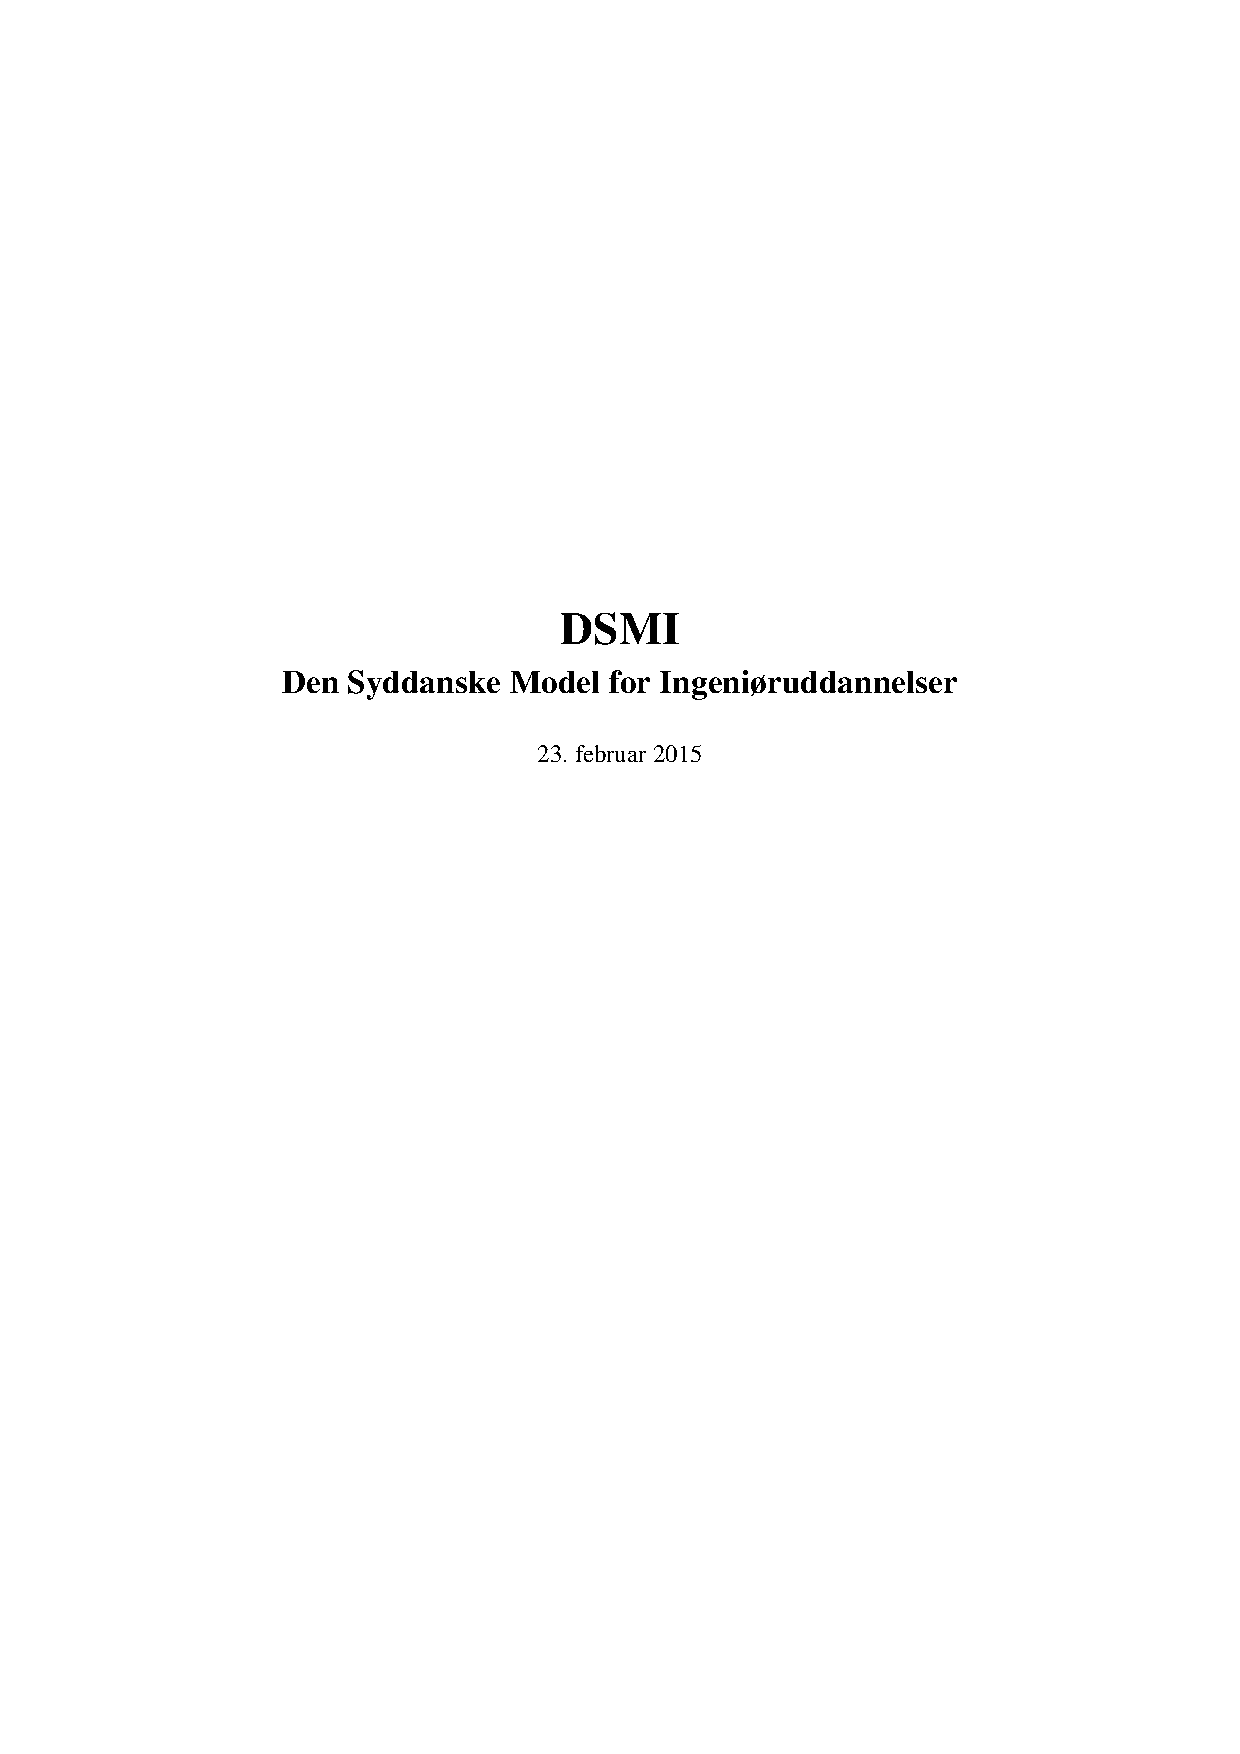
\includepdf[pages=-,pagecommand={} \label{sec:DSMI}]{pdfs/DSMI 23 februar 2015.pdf}
}
\end{document}